\section{Uppgift 8}\label{uppgift-8}

\subsection{Instruktioner}
\begin{verbatim}
8. Skriv ett program som skriver ut en viss multiplikationstabell. Den som kör
   programmet ska ange önskad multiplikationstabell och hur långt programmet ska
   räkna. Exempel på utskrift om man väljer tabell 8 och upp till 4:

    Vilken mulitiplikationstabell önskas? *8*
    Hur långt ska jag räkna? *4*

    8 * 1 = 8
    8 * 2 = 16
    8 * 3 = 24
    8 * 4 = 32
\end{verbatim}

\subsection{Lösning}
\subsubsection{Funktion}
% TODO: Funktion på %8.
\subsubsection{Kommentar}
% TODO: Kommentar på %8.

\subsubsection{Källkod}\label{uppgift-8_src}
%\begin{listing}[H]
    \inputminted[linenos]{java}{src/Lab1Uppg08.java}
    \caption{Lab1Uppg08.java}
    \label{Uppg8src}
%\end{listing}

\subsubsection{Skärmdump}
\begin{figure}[htbp]
    \centering
        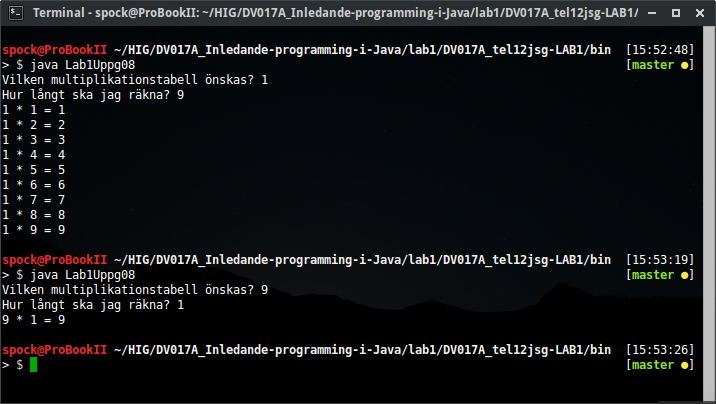
\includegraphics[width=\linewidth]{img/08.png}
    \caption{Körning av koden till Uppgift \ref{uppgift-8}}
    \label{fig:screenshot-08}
\end{figure}
